\documentclass[12pt]{extarticle}
\usepackage[english, russian]{babel}
\usepackage[left=20mm, right=10mm, top=20mm, bottom=20mm]{geometry}
\usepackage{graphicx}
\usepackage{titlesec}
\usepackage{array}
\usepackage{wrapfig}
\usepackage{color, colortbl}
\usepackage[colorlinks=true,linkcolor=cyan,unicode=true]{hyperref}
\usepackage{mathtools}
\usepackage{setspace}
\usepackage{svg}
\usepackage{amssymb}
 
\newcommand\ddformula[1]{\displaystyle #1}
 
\titleformat{\section}
  {\normalfont\fontsize{12}{14}\bfseries}{\thesection}{0.5em}{}
 
\begin{document}
    \begin{minipage}{0.5\textwidth}
        \begin{center}
            \begin{small}
                \textsf{\textbf{Университет ИТМО}} \\
                \textsf{\textbf{Физико-технический мегафакультет}} \\
                \textsf{\textbf{Физический факультет}}
            \end{small}
        \end{center}
    \end{minipage}
    \hfill
    \begin{minipage}{0.4\textwidth}
        
\includegraphics[height=2.5cm]{itmo.png}
    \end{minipage}
    \hrule
    \vspace{8mm}
    \begin{minipage}{0.4\textwidth}
        Группа: P3208 \\ % ГРУППА
        Студент: Ходжаев А.А. \\ % СТУДЕНТ
        Преподаватель: Смирнов А.В % ПРЕПОД
    \end{minipage}
    \hfill
    \begin{minipage}{0.4\textwidth}
        К работе допущен: \\
        Работа выполнена: \\
        Отчёт принят: 
    \end{minipage}
    \vspace{8mm}
    \begin{center}
        \begin{Large}
            \textbf{Рабочий протокол и отчёт по лабораторной работе №3.01} \\ % УКАЗАТЬ НОМЕР ЛАБЫ
            Изучение электростатического поля методом моделирования % УКАЗАТЬ НАЗВАНИЕ ЛАБЫ
        \end{Large}
    \end{center}
    \vspace{8mm}
 
    \section{Цель работы}
    Изучить электростатическое поле, построив сечения эквипотенциальных поверхностей и силовых линий электростатического поля на основе экспериментального моделирования распределения потенциала в слабопроводящей среде

    \section{Задачи, решаемые при выполнении работы}
    1. Изобразить данные измерений на масштабно-координатную бумагу
    \\2. Построить сечения эквипотенциальных поверхностей и силовых линий электростатического поля
    \\3. Проанализовать данные
    \\4. Провести косвенные вычисления
    \\5. Построить графики зависимостей $\varphi = \varphi(x)$
    
    \section{Объект исследования}
    Потенциал в слабопроводящей среде

    \section{Метод экспериментального исследования}
    Эксперимент. Размещение в слабопроводящей среде электродов для построения сечений эквипотенциальных поверхностей и силовых линий

    \section{Рабочие формулы и исходные данные}
    
    Средняя напряженность
    \begin{equation*}
        \langle E_{12} \rangle \approxeq A \frac{\varphi_1 - \varphi_2}{l_{12}}
    \end{equation*}
    где $l_{12}$ - длина участка силовой линии между точками, 
    $\varphi_1$ и $\varphi_2$ потенциалы двух точек, лежащих на одной силовой линии
    \\
    Поверхностная плотность зарядов
    \begin{equation*}
        \sigma^\prime \approxeq -\varepsilon_0 \frac{\Delta\varphi}{\Delta l_n}
    \end{equation*}
    где $\Delta\varphi$ - изменение потенциала при смещении на малое расстояние $\Delta l_n$
    \section{Измерительные приборы}
    \begin{tabular}{|p{1cm}|p{4cm}|p{5cm}|p{3cm}|p{3cm}|}
        \hline
        \textbf{№} & \textbf{Наименование} & \textbf{Тип прибора} & \textbf{Используемый диапазон} & \textbf{Погрешность прибора} \\ \hline
        1 & Вольтметр & Измерение потенциала & 0 - 20 В & 0.001 В \\ \hline
        2 & Линейка & Ось абцисс & 2-28 см & 1 мм \\ \hline
        3 & линейка & Ось ординат & 2-18 см & 1 мм \\
        \hline
    \end{tabular}
    
    \section{Схема установки}
    \begin{minipage}{0.5\textwidth}
        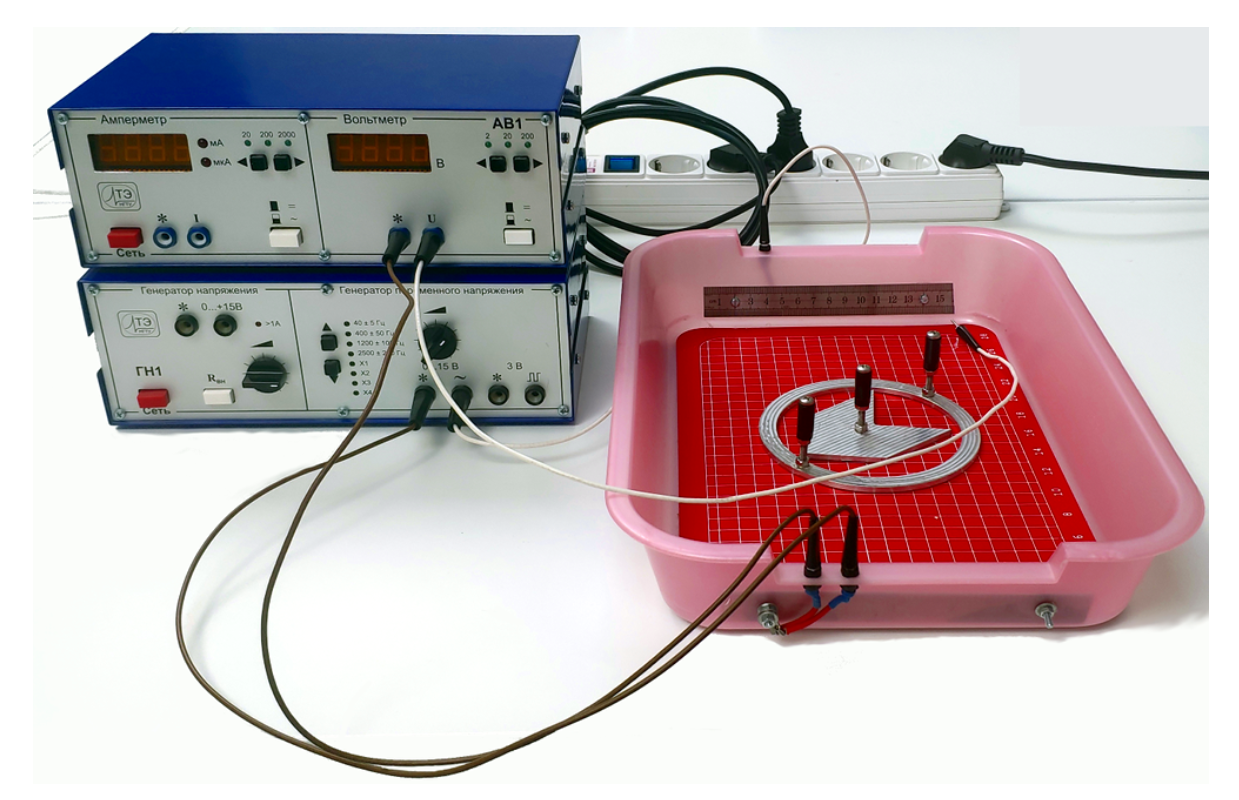
\includegraphics[height=7cm]{image.png}
    \end{minipage}
    \hfill
    \begin{minipage}{0.4\textwidth}
        На боковых стенках электролитичtской ванны
        расположены плоские металлические электроды,
        подключенные к многофункциональному генератору напряжения ГН1.
        Между электродами находится измерительный зонд в виде 
        тонкого изолированного проводника, подсоединенного к вольтметру.
        Вольтметр в составе комбинированного прибора АВ1 показывает
        действующую разность потенциалов между зондом и электродом,
        подключенным ко второму гнезду вольтметра. Собственное 
        сопротивление вольтметра существенно превышает сопротивление
        воды в ванне, для того чтобы измерительный ток вольтметра не
        шунтировал токи в модели и не искажал распределение электрического поля
    \end{minipage}

    \section{Результаты прямых измерений}

    \section{Расчёт результатов косвенных изменений}

    \section{Расчёт погрешностей изменений}
 
    \section{Графики}

    \section{Окончательные результаты}

    \section{Вывод и анализ результатов}

    \end{document}